% \addcontentsline{toc}{chapter}{Conclusioni}
% \chapter*{Conclusioni}
\chapter{Simulazioni}
\label{chap:cap4}
Come già accennato nel primo capitolo, in questo lavoro di tesi ci siamo serviti di Netlogo al fine di costruire un modello di diffusione epidemica su rete; in particolare, abbiamo fatto uso di BehaviorSpace, un software, messo a disposizione da Netlogo stesso, che consente di eseguire più volte un esperimento andandone a variare alcuni parametri caratteristici \cite{Wilensky2}. 
\section{Il modello}
Il nostro obiettivo è quello di andare a valutare come varia la frazione di individui che non contraggono mai l'infezione al mutare della percezione del rischio; al suo aumentare ci aspettiamo, abbastanza intuitivamente, che il processo diffusivo si arresti prima e che, quindi, il numero di soggetti che non si sono ammalati diventi via via maggiore. \\Il modello compartimentale preso in considerazione è il SIS (suscettibili-infetti-suscettibili), che non prevede l'acquisizione di alcun tipo di immunità una volta guariti dall'infezione \cite{Brauer}. Affinché fosse più immediato visualizzarne l'evoluzione nel tempo, abbiamo generato una rete con un numero di nodi ("num- che poteva variare da un minimo di $ 2 $ ad un massimo di $ 1000 $; si è scelto di mantenere l'indicatore su di questo ultimo valore per tutte le simulazioni condotte. \`{E} stato anche possibile controllare mediante slider ("preferential-attachment") la probabilità che un nuovo nodo risultasse legato ad un altro già altamente connesso: ciò ha consentito di dare origine sia a reti totalmente aleatorie, che a reti di tipo scale-free. \\Altri parametri presi in considerazione - anch'essi modificabili tramite un cursore - sono stati:
\begin{itemize}
\item \textit{la frazione iniziale di infetti} ("fraction-infected");
\item \textit{il tasso di infettività} ("infectivity");
\item \textit{il livello di misure di precauzione} individuali, indicato genericamente come "risk-perception", ma coincidente con la quantità $ J $ definita nel precedente capitolo.
\end{itemize}
\begin{figure}[t]
		\begin{center}
			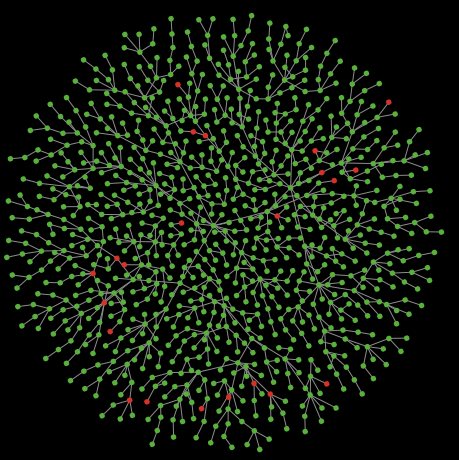
\includegraphics[scale=.6, keepaspectratio]{network_w_Netlogo_1}
			\caption{Esempio di rete generata col programma su Netlogo dopo aver impostato "num-nodes" $= 1000 $, "preferential-attachment $= 0.00 $ e "infected-fraction" $= 0.031 $.}
			\label{fig:NetLogo1}
		\end{center}
\end{figure}
%Ricordiamo, a questo proposito, di aver sostituito alla probabilità di infezione netta $ \tau $ il prodotto $ \tau \cdot exp(-J \tfrac{s}{k}) $, dove con $ \tfrac{s}{k} $ si è indicato la frazione $ s $ di infetti su $ k $ vicini; nel codice sviluppato questa quantità è stata resa dalla variabile "alert" 
Gli agenti - che su NetLogo vengono indicati con il nome di \emph{turtles} - possono essere descritti in termini di tre variabili:
\begin{enumerate}
\item \textit{"state"}, alla quale viene assegnato un valore numerico $ \geq 0 $ sulla base della condizione di salute e che, pertanto, funge da contatore per la durata del periodo d'infezione;
\item \textit{infected?}, che può assumere valore vero/falso;
\item \textit{alert}, che tiene conto della quantità di vicini infetti (quella che, nel precedente capitolo, veniva indicata come $ \tfrac{s}{k}$).
\end{enumerate}
Come viene reso evidente in \cref{fig:NetLogo1}, i nodi di colore rosso sono quelli infetti; il loro numero viene stabilito a seguito dell'estrazione di un numero casuale fra $ 0 $ e $ 1 $ e del confronto di questo con la quantità "initial-infected". La probabilità che contagino i vertici ai quali sono collegati è anch'essa aleatoria:
\begin{center}
	\begin{lstlisting}[language={NetLogo},caption={Porzione di codice in cui si mette in luce il meccanismo di infezione},label={list:infection_prob}]
		ask turtles with [state > 0] [
    		ask out-link-neighbors with [state = 0] [
      			if random-float 1 < infectivity * exp(-1 * risk-perception * alert) [
        				set state num-states
        				set infected? true
      			]
    		]
  		]
	\end{lstlisting}
\end{center}
Rimandiamo all'appendice \ref{appendix:code} per il codice sviluppato.


	
	